\documentclass[letterpaper,12pt]{article}
\usepackage[margin=14mm,top=18mm,bottom=17mm,headheight=14pt]{geometry}
\pdfmapfile{+cm.map}\pdfmapfile{+cmextra.map}
\usepackage{tikz,fancyhdr,amsmath,amssymb}
\usetikzlibrary{arrows.meta,patterns}
\pagestyle{fancy}\fancyhf{}\renewcommand{\headrulewidth}{0pt}
\fancyhead[L]{\small Week 47 / Gentle-step landscapes / K--1}
\fancyfoot[L]{\small Bellingham Math Circle / Week 47 / F47-K-v3}
\fancyfoot[R]{\small\thepage}
\setlength{\parindent}{0pt}\setlength{\parskip}{0pt}
\begin{document}
\noindent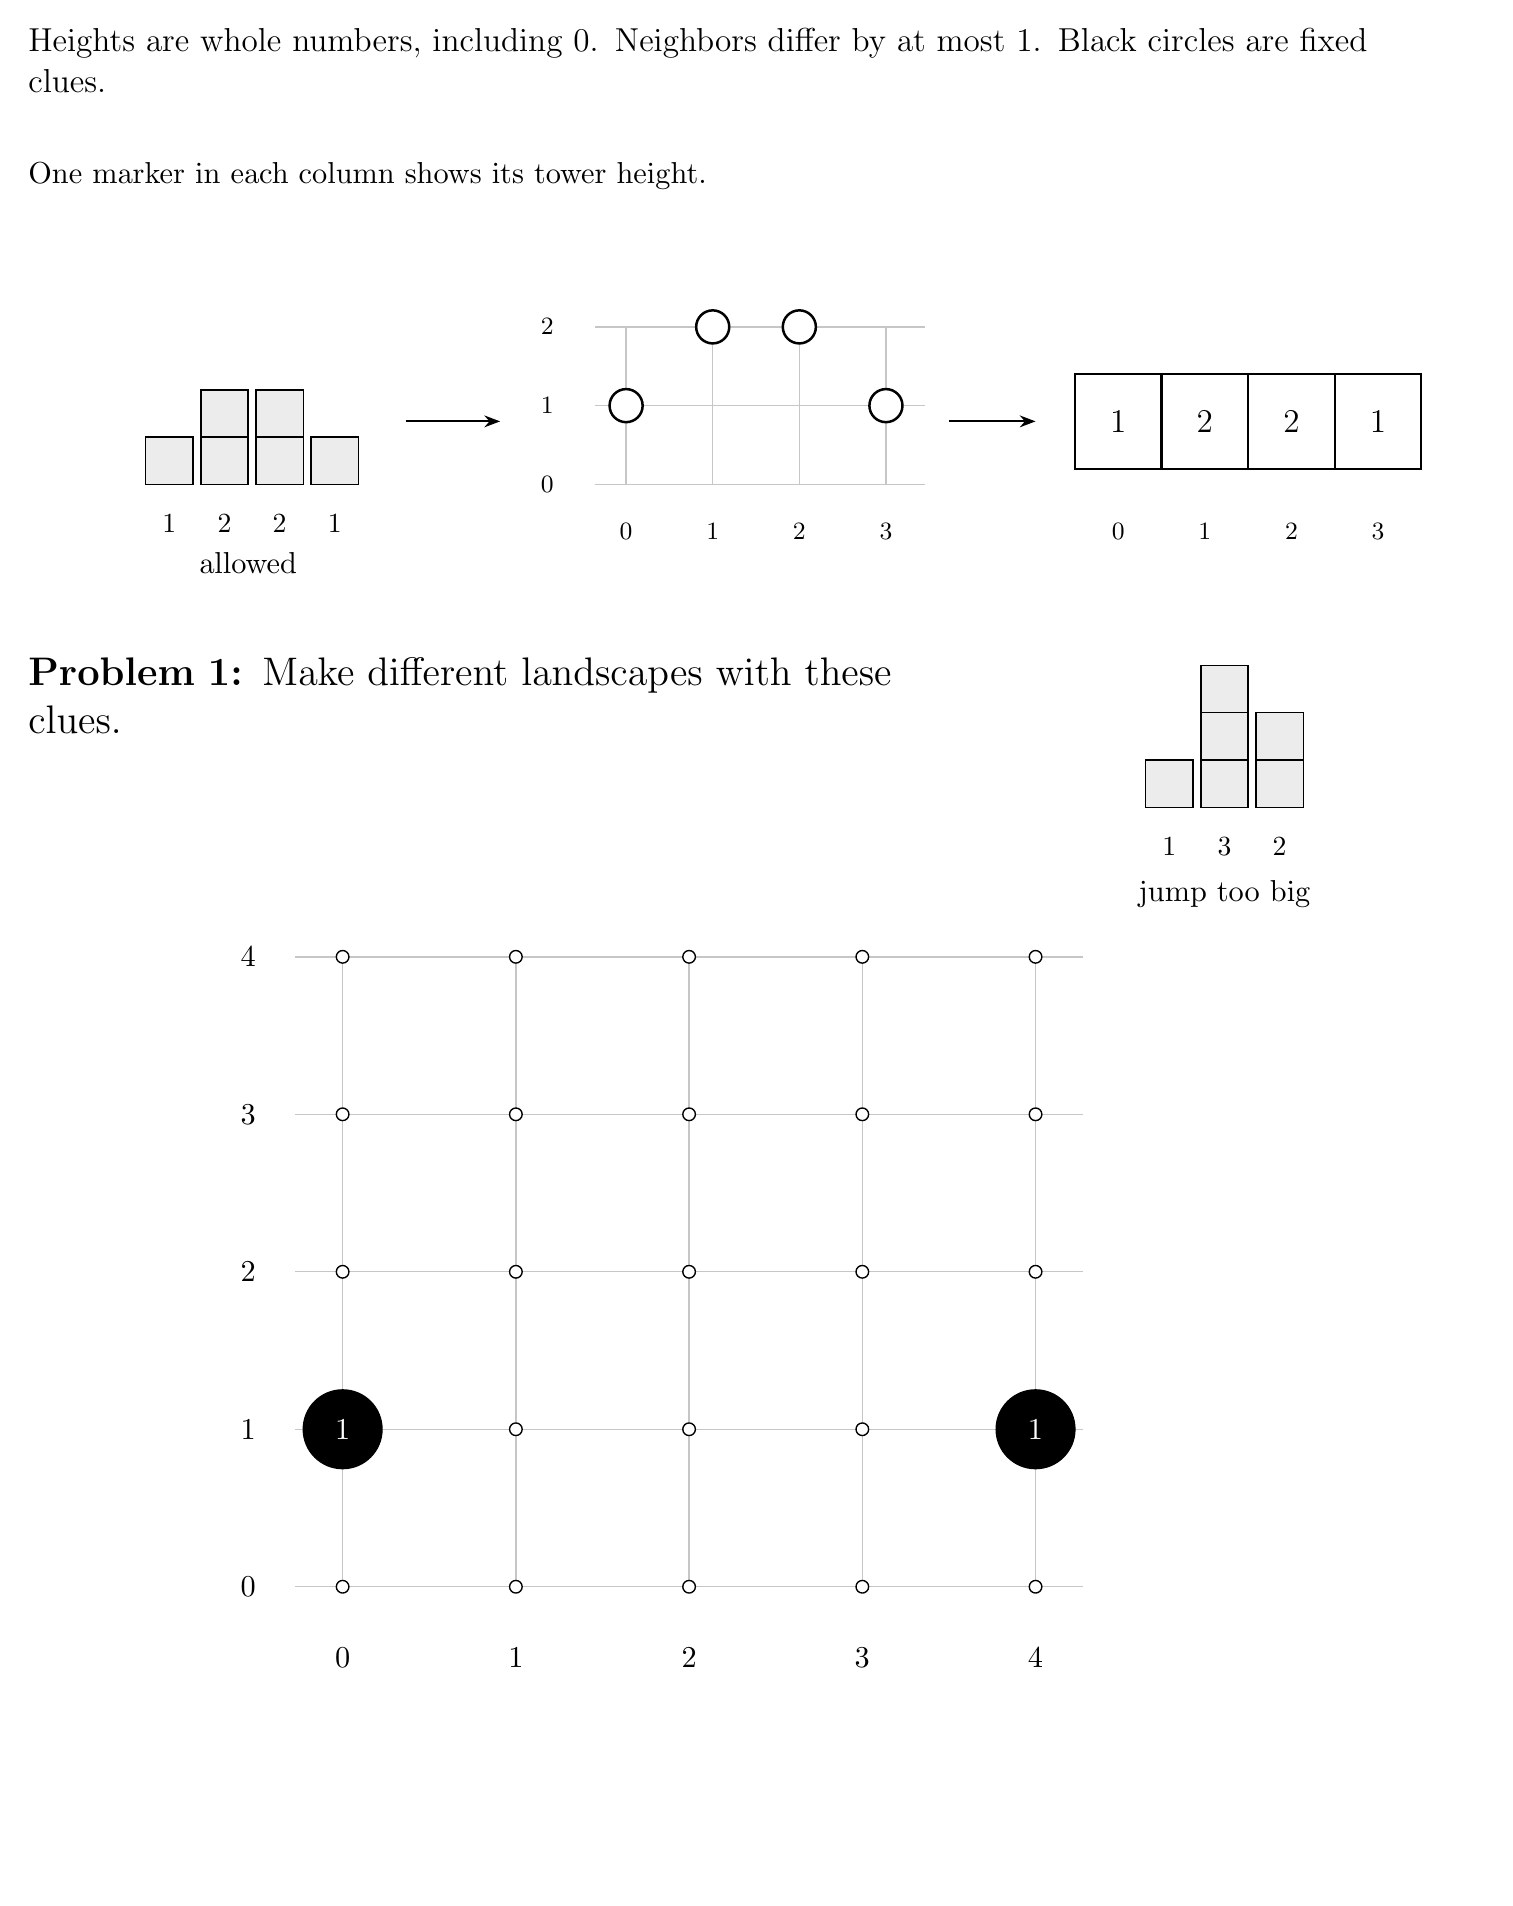
\begin{tikzpicture}[x=1mm,y=-1mm,line width=.5pt]
\path[use as bounding box] (0,0) rectangle (185,235);
\node[anchor=north west,inner sep=0pt,text width=180mm,font=\fontsize{12}{15}\selectfont] at (0,0) {Heights are whole numbers, including 0. Neighbors differ by at most 1. Black circles are fixed clues.};
\node[anchor=north west,inner sep=0pt,text width=180mm,font=\fontsize{11}{14}\selectfont] at (0,17) {One marker in each column shows its tower height.};
\draw[fill=gray!15] (15,52) rectangle ++(6,6);
\node[anchor=center,inner sep=1pt,font=\fontsize{10}{12}\selectfont] at (18.0,63) {1};
\draw[fill=gray!15] (22,52) rectangle ++(6,6);
\draw[fill=gray!15] (22,46) rectangle ++(6,6);
\node[anchor=center,inner sep=1pt,font=\fontsize{10}{12}\selectfont] at (25.0,63) {2};
\draw[fill=gray!15] (29,52) rectangle ++(6,6);
\draw[fill=gray!15] (29,46) rectangle ++(6,6);
\node[anchor=center,inner sep=1pt,font=\fontsize{10}{12}\selectfont] at (32.0,63) {2};
\draw[fill=gray!15] (36,52) rectangle ++(6,6);
\node[anchor=center,inner sep=1pt,font=\fontsize{10}{12}\selectfont] at (39.0,63) {1};
\node[anchor=center,inner sep=1pt,font=\fontsize{11}{13}\selectfont] at (28,68) {allowed};
\draw[gray!45] (72,58) -- (114,58);
\node[anchor=center,inner sep=1pt,font=\fontsize{9}{11}\selectfont] at (66,58) {0};
\draw[gray!45] (72,48) -- (114,48);
\node[anchor=center,inner sep=1pt,font=\fontsize{9}{11}\selectfont] at (66,48) {1};
\draw[gray!45] (72,38) -- (114,38);
\node[anchor=center,inner sep=1pt,font=\fontsize{9}{11}\selectfont] at (66,38) {2};
\draw[gray!45] (76,38) -- (76,58);
\draw[fill=white,line width=.9pt] (76,48) circle (2.1);
\node[anchor=center,inner sep=1pt,font=\fontsize{9}{11}\selectfont] at (76,64) {0};
\draw[gray!45] (87,38) -- (87,58);
\draw[fill=white,line width=.9pt] (87,38) circle (2.1);
\node[anchor=center,inner sep=1pt,font=\fontsize{9}{11}\selectfont] at (87,64) {1};
\draw[gray!45] (98,38) -- (98,58);
\draw[fill=white,line width=.9pt] (98,38) circle (2.1);
\node[anchor=center,inner sep=1pt,font=\fontsize{9}{11}\selectfont] at (98,64) {2};
\draw[gray!45] (109,38) -- (109,58);
\draw[fill=white,line width=.9pt] (109,48) circle (2.1);
\node[anchor=center,inner sep=1pt,font=\fontsize{9}{11}\selectfont] at (109,64) {3};
\draw[-{Stealth[length=2mm]},line width=.8pt] (48,50) -- (60,50);
\draw[-{Stealth[length=2mm]},line width=.8pt] (117,50) -- (128,50);
\draw[line width=.8pt] (133,44) rectangle ++(44,12);
\node[anchor=center,inner sep=1pt,font=\fontsize{13}{15}\selectfont] at (138.5,50) {1};
\node[anchor=center,inner sep=1pt,font=\fontsize{9}{11}\selectfont] at (138.5,64) {0};
\draw[line width=.8pt] (144,44) -- (144,56);
\node[anchor=center,inner sep=1pt,font=\fontsize{13}{15}\selectfont] at (149.5,50) {2};
\node[anchor=center,inner sep=1pt,font=\fontsize{9}{11}\selectfont] at (149.5,64) {1};
\draw[line width=.8pt] (155,44) -- (155,56);
\node[anchor=center,inner sep=1pt,font=\fontsize{13}{15}\selectfont] at (160.5,50) {2};
\node[anchor=center,inner sep=1pt,font=\fontsize{9}{11}\selectfont] at (160.5,64) {2};
\draw[line width=.8pt] (166,44) -- (166,56);
\node[anchor=center,inner sep=1pt,font=\fontsize{13}{15}\selectfont] at (171.5,50) {1};
\node[anchor=center,inner sep=1pt,font=\fontsize{9}{11}\selectfont] at (171.5,64) {3};
\node[anchor=north west,inner sep=0pt,text width=113mm,font=\fontsize{14}{17}\selectfont] at (0,80) {\textbf{Problem 1:} Make different landscapes with these clues.};
\draw[fill=gray!15] (142,93) rectangle ++(6,6);
\node[anchor=center,inner sep=1pt,font=\fontsize{10}{12}\selectfont] at (145.0,104) {1};
\draw[fill=gray!15] (149,93) rectangle ++(6,6);
\draw[fill=gray!15] (149,87) rectangle ++(6,6);
\draw[fill=gray!15] (149,81) rectangle ++(6,6);
\node[anchor=center,inner sep=1pt,font=\fontsize{10}{12}\selectfont] at (152.0,104) {3};
\draw[fill=gray!15] (156,93) rectangle ++(6,6);
\draw[fill=gray!15] (156,87) rectangle ++(6,6);
\node[anchor=center,inner sep=1pt,font=\fontsize{10}{12}\selectfont] at (159.0,104) {2};
\node[anchor=center,inner sep=1pt,font=\fontsize{11}{13}\selectfont] at (152,110) {jump too big};
\draw[gray!45] (34,198) -- (134,198);
\node[anchor=center,inner sep=1pt,font=\fontsize{11}{13}\selectfont] at (28,198) {0};
\draw[gray!45] (34,178) -- (134,178);
\node[anchor=center,inner sep=1pt,font=\fontsize{11}{13}\selectfont] at (28,178) {1};
\draw[gray!45] (34,158) -- (134,158);
\node[anchor=center,inner sep=1pt,font=\fontsize{11}{13}\selectfont] at (28,158) {2};
\draw[gray!45] (34,138) -- (134,138);
\node[anchor=center,inner sep=1pt,font=\fontsize{11}{13}\selectfont] at (28,138) {3};
\draw[gray!45] (34,118) -- (134,118);
\node[anchor=center,inner sep=1pt,font=\fontsize{11}{13}\selectfont] at (28,118) {4};
\draw[gray!45] (40,118) -- (40,198);
\draw[fill=white] (40,198) circle (0.8);
\draw[fill=white] (40,178) circle (0.8);
\draw[fill=white] (40,158) circle (0.8);
\draw[fill=white] (40,138) circle (0.8);
\draw[fill=white] (40,118) circle (0.8);
\node[anchor=center,inner sep=1pt,font=\fontsize{11}{13}\selectfont] at (40,207) {0};
\draw[fill=black] (40,178) circle (5);
\node[anchor=center,inner sep=1pt,font=\fontsize{11}{13}\selectfont] at (40,178) {\color{white}1};
\draw[gray!45] (62,118) -- (62,198);
\draw[fill=white] (62,198) circle (0.8);
\draw[fill=white] (62,178) circle (0.8);
\draw[fill=white] (62,158) circle (0.8);
\draw[fill=white] (62,138) circle (0.8);
\draw[fill=white] (62,118) circle (0.8);
\node[anchor=center,inner sep=1pt,font=\fontsize{11}{13}\selectfont] at (62,207) {1};
\draw[gray!45] (84,118) -- (84,198);
\draw[fill=white] (84,198) circle (0.8);
\draw[fill=white] (84,178) circle (0.8);
\draw[fill=white] (84,158) circle (0.8);
\draw[fill=white] (84,138) circle (0.8);
\draw[fill=white] (84,118) circle (0.8);
\node[anchor=center,inner sep=1pt,font=\fontsize{11}{13}\selectfont] at (84,207) {2};
\draw[gray!45] (106,118) -- (106,198);
\draw[fill=white] (106,198) circle (0.8);
\draw[fill=white] (106,178) circle (0.8);
\draw[fill=white] (106,158) circle (0.8);
\draw[fill=white] (106,138) circle (0.8);
\draw[fill=white] (106,118) circle (0.8);
\node[anchor=center,inner sep=1pt,font=\fontsize{11}{13}\selectfont] at (106,207) {3};
\draw[gray!45] (128,118) -- (128,198);
\draw[fill=white] (128,198) circle (0.8);
\draw[fill=white] (128,178) circle (0.8);
\draw[fill=white] (128,158) circle (0.8);
\draw[fill=white] (128,138) circle (0.8);
\draw[fill=white] (128,118) circle (0.8);
\node[anchor=center,inner sep=1pt,font=\fontsize{11}{13}\selectfont] at (128,207) {4};
\draw[fill=black] (128,178) circle (5);
\node[anchor=center,inner sep=1pt,font=\fontsize{11}{13}\selectfont] at (128,178) {\color{white}1};
\end{tikzpicture}
\newpage
\noindent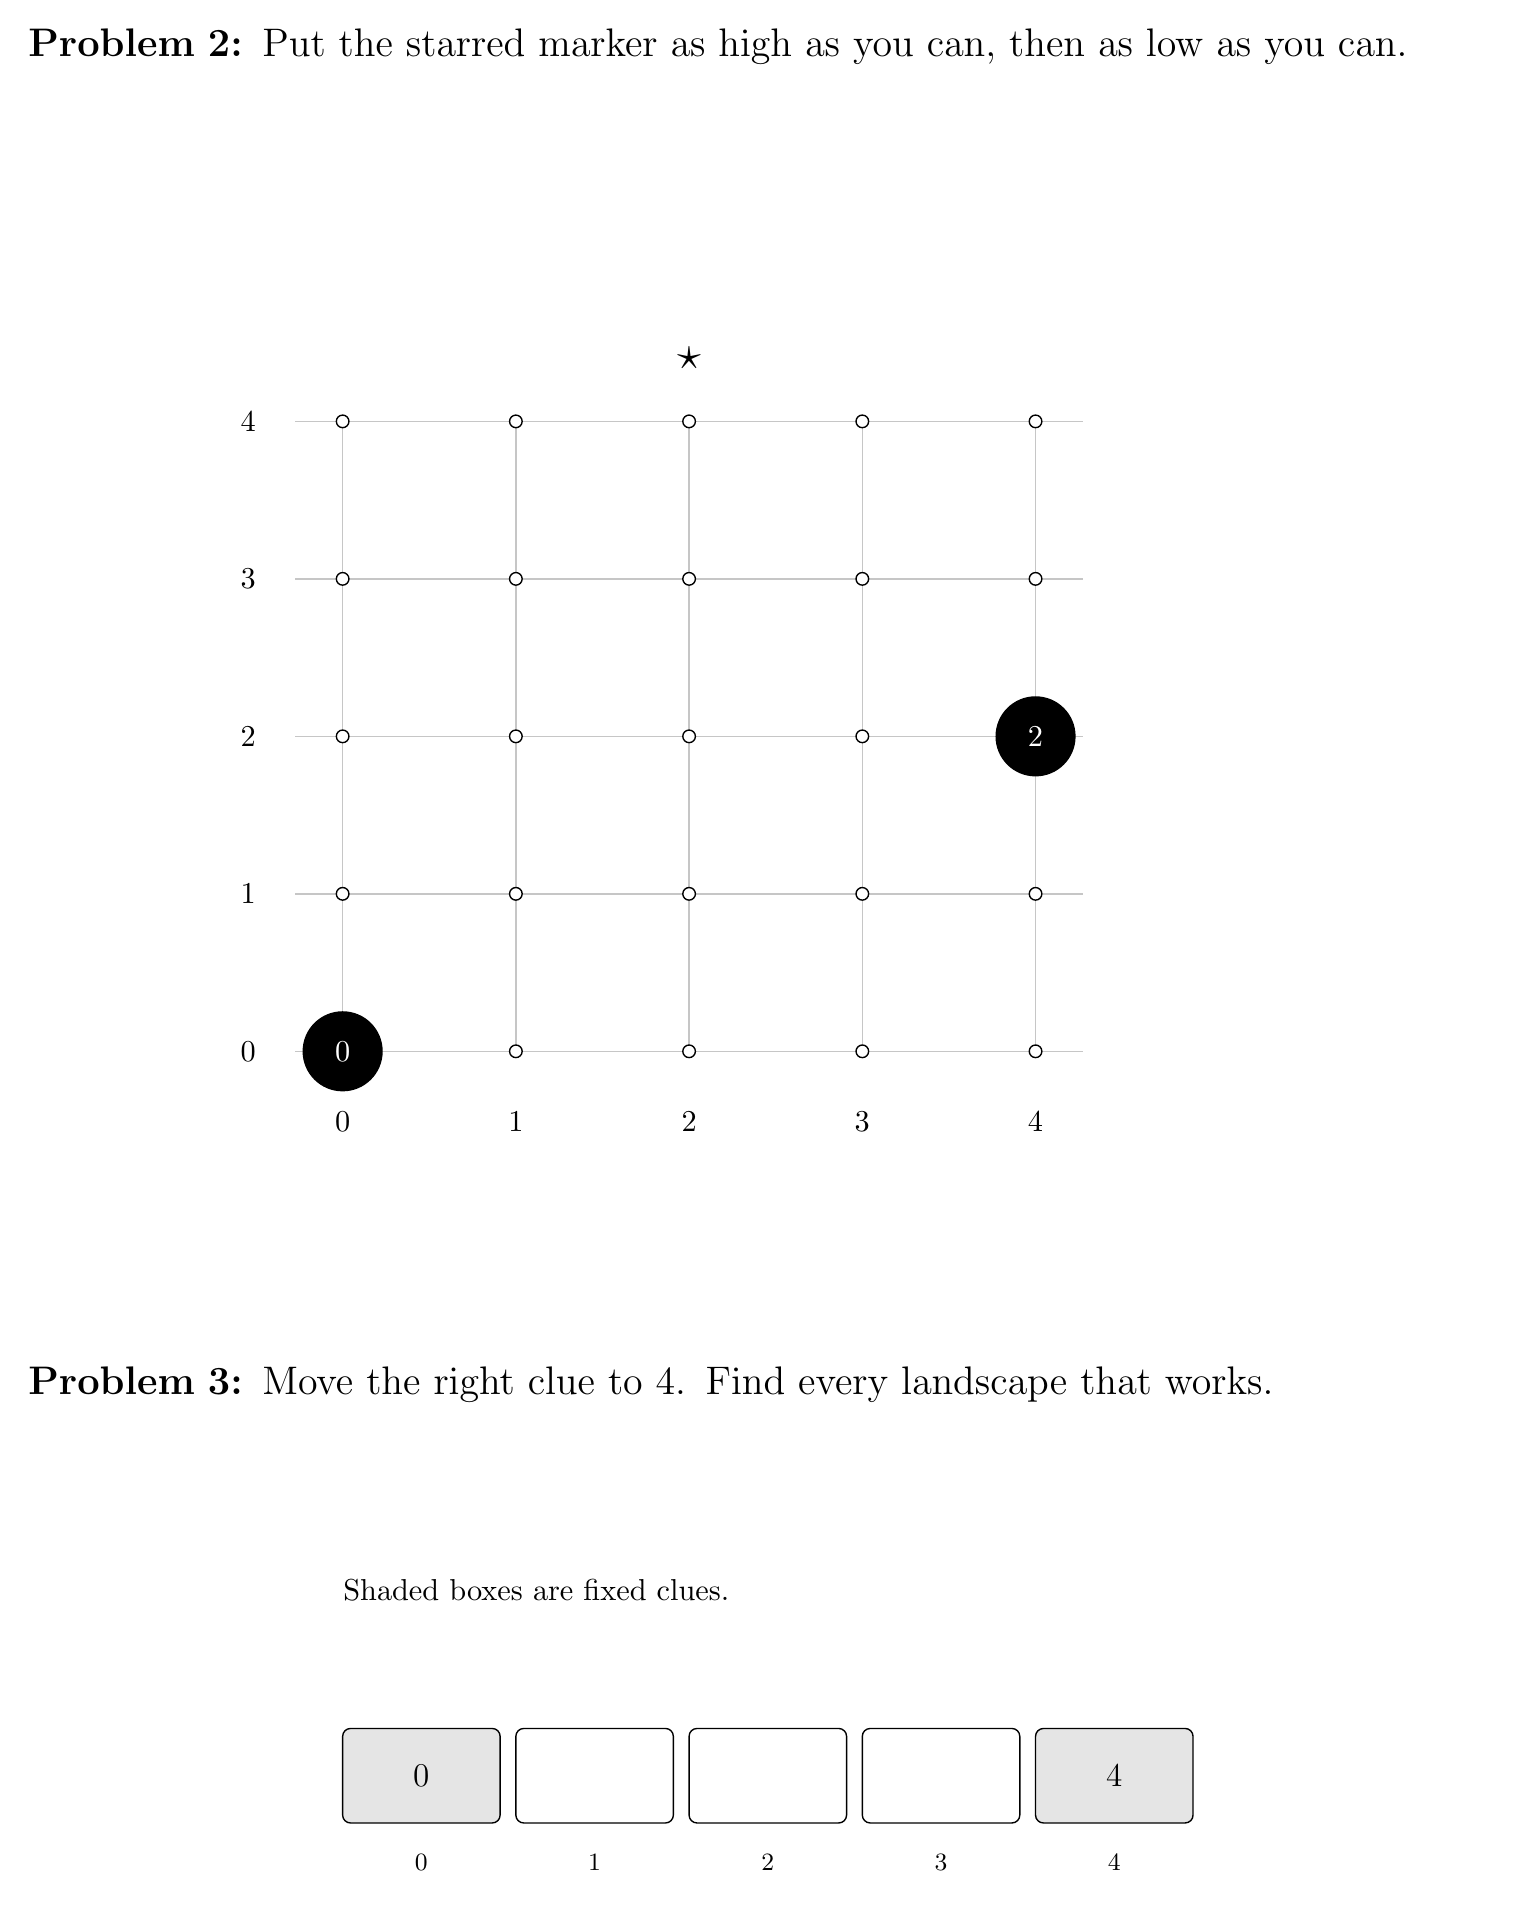
\begin{tikzpicture}[x=1mm,y=-1mm,line width=.5pt]
\path[use as bounding box] (0,0) rectangle (185,235);
\node[anchor=north west,inner sep=0pt,text width=180mm,font=\fontsize{14}{17}\selectfont] at (0,0) {\textbf{Problem 2:} Put the starred marker as high as you can, then as low as you can.};
\draw[gray!45] (34,130) -- (134,130);
\node[anchor=center,inner sep=1pt,font=\fontsize{11}{13}\selectfont] at (28,130) {0};
\draw[gray!45] (34,110) -- (134,110);
\node[anchor=center,inner sep=1pt,font=\fontsize{11}{13}\selectfont] at (28,110) {1};
\draw[gray!45] (34,90) -- (134,90);
\node[anchor=center,inner sep=1pt,font=\fontsize{11}{13}\selectfont] at (28,90) {2};
\draw[gray!45] (34,70) -- (134,70);
\node[anchor=center,inner sep=1pt,font=\fontsize{11}{13}\selectfont] at (28,70) {3};
\draw[gray!45] (34,50) -- (134,50);
\node[anchor=center,inner sep=1pt,font=\fontsize{11}{13}\selectfont] at (28,50) {4};
\draw[gray!45] (40,50) -- (40,130);
\draw[fill=white] (40,130) circle (0.8);
\draw[fill=white] (40,110) circle (0.8);
\draw[fill=white] (40,90) circle (0.8);
\draw[fill=white] (40,70) circle (0.8);
\draw[fill=white] (40,50) circle (0.8);
\node[anchor=center,inner sep=1pt,font=\fontsize{11}{13}\selectfont] at (40,139) {0};
\draw[fill=black] (40,130) circle (5);
\node[anchor=center,inner sep=1pt,font=\fontsize{11}{13}\selectfont] at (40,130) {\color{white}0};
\draw[gray!45] (62,50) -- (62,130);
\draw[fill=white] (62,130) circle (0.8);
\draw[fill=white] (62,110) circle (0.8);
\draw[fill=white] (62,90) circle (0.8);
\draw[fill=white] (62,70) circle (0.8);
\draw[fill=white] (62,50) circle (0.8);
\node[anchor=center,inner sep=1pt,font=\fontsize{11}{13}\selectfont] at (62,139) {1};
\draw[gray!45] (84,50) -- (84,130);
\draw[fill=white] (84,130) circle (0.8);
\draw[fill=white] (84,110) circle (0.8);
\draw[fill=white] (84,90) circle (0.8);
\draw[fill=white] (84,70) circle (0.8);
\draw[fill=white] (84,50) circle (0.8);
\node[anchor=center,inner sep=1pt,font=\fontsize{11}{13}\selectfont] at (84,139) {2};
\node[anchor=center,inner sep=1pt,font=\fontsize{16}{18}\selectfont] at (84,42) {$\star$};
\draw[gray!45] (106,50) -- (106,130);
\draw[fill=white] (106,130) circle (0.8);
\draw[fill=white] (106,110) circle (0.8);
\draw[fill=white] (106,90) circle (0.8);
\draw[fill=white] (106,70) circle (0.8);
\draw[fill=white] (106,50) circle (0.8);
\node[anchor=center,inner sep=1pt,font=\fontsize{11}{13}\selectfont] at (106,139) {3};
\draw[gray!45] (128,50) -- (128,130);
\draw[fill=white] (128,130) circle (0.8);
\draw[fill=white] (128,110) circle (0.8);
\draw[fill=white] (128,90) circle (0.8);
\draw[fill=white] (128,70) circle (0.8);
\draw[fill=white] (128,50) circle (0.8);
\node[anchor=center,inner sep=1pt,font=\fontsize{11}{13}\selectfont] at (128,139) {4};
\draw[fill=black] (128,90) circle (5);
\node[anchor=center,inner sep=1pt,font=\fontsize{11}{13}\selectfont] at (128,90) {\color{white}2};
\node[anchor=north west,inner sep=0pt,text width=180mm,font=\fontsize{14}{17}\selectfont] at (0,170) {\textbf{Problem 3:} Move the right clue to 4. Find every landscape that works.};
\node[anchor=north west,inner sep=0pt,text width=140mm,font=\fontsize{11}{14}\selectfont] at (40,197) {Shaded boxes are fixed clues.};
\draw[rounded corners=1mm,fill=gray!20] (40,216) rectangle ++(20,12);
\node[anchor=center,inner sep=1pt,font=\fontsize{13}{15}\selectfont] at (50.0,222) {0};
\node[anchor=center,inner sep=1pt,font=\fontsize{9}{11}\selectfont] at (50.0,233) {0};
\draw[rounded corners=1mm] (62,216) rectangle ++(20,12);
\node[anchor=center,inner sep=1pt,font=\fontsize{13}{15}\selectfont] at (72.0,222) {};
\node[anchor=center,inner sep=1pt,font=\fontsize{9}{11}\selectfont] at (72.0,233) {1};
\draw[rounded corners=1mm] (84,216) rectangle ++(20,12);
\node[anchor=center,inner sep=1pt,font=\fontsize{13}{15}\selectfont] at (94.0,222) {};
\node[anchor=center,inner sep=1pt,font=\fontsize{9}{11}\selectfont] at (94.0,233) {2};
\draw[rounded corners=1mm] (106,216) rectangle ++(20,12);
\node[anchor=center,inner sep=1pt,font=\fontsize{13}{15}\selectfont] at (116.0,222) {};
\node[anchor=center,inner sep=1pt,font=\fontsize{9}{11}\selectfont] at (116.0,233) {3};
\draw[rounded corners=1mm,fill=gray!20] (128,216) rectangle ++(20,12);
\node[anchor=center,inner sep=1pt,font=\fontsize{13}{15}\selectfont] at (138.0,222) {4};
\node[anchor=center,inner sep=1pt,font=\fontsize{9}{11}\selectfont] at (138.0,233) {4};
\end{tikzpicture}
\newpage
\noindent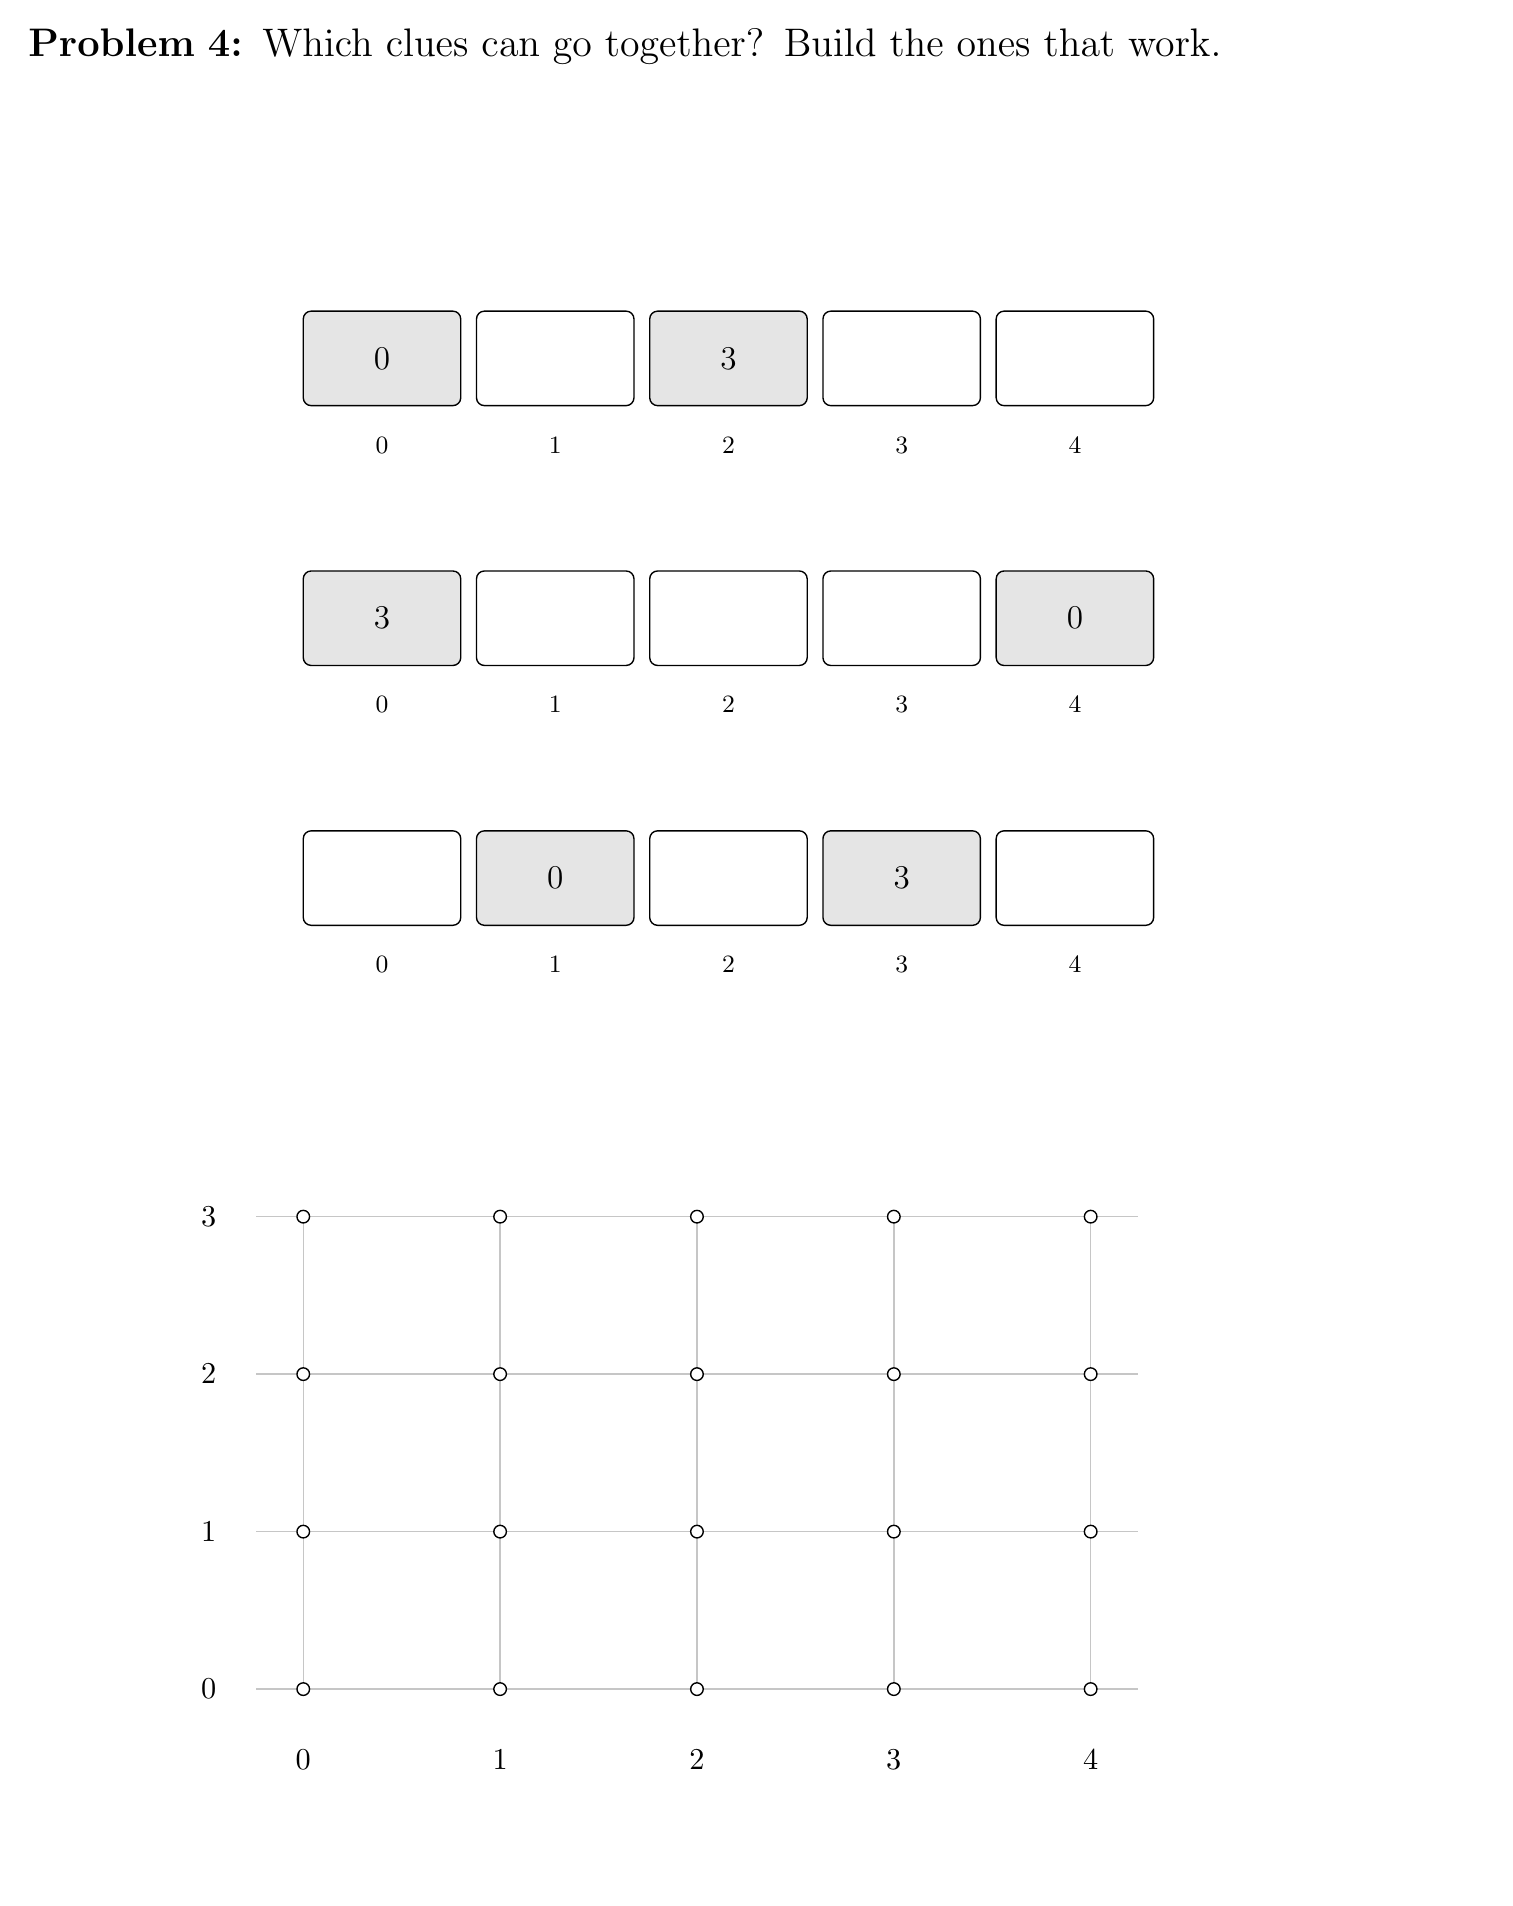
\begin{tikzpicture}[x=1mm,y=-1mm,line width=.5pt]
\path[use as bounding box] (0,0) rectangle (185,235);
\node[anchor=north west,inner sep=0pt,text width=180mm,font=\fontsize{14}{17}\selectfont] at (0,0) {\textbf{Problem 4:} Which clues can go together? Build the ones that work.};
\draw[rounded corners=1mm,fill=gray!20] (35,36) rectangle ++(20,12);
\node[anchor=center,inner sep=1pt,font=\fontsize{13}{15}\selectfont] at (45.0,42) {0};
\node[anchor=center,inner sep=1pt,font=\fontsize{9}{11}\selectfont] at (45.0,53) {0};
\draw[rounded corners=1mm] (57,36) rectangle ++(20,12);
\node[anchor=center,inner sep=1pt,font=\fontsize{13}{15}\selectfont] at (67.0,42) {};
\node[anchor=center,inner sep=1pt,font=\fontsize{9}{11}\selectfont] at (67.0,53) {1};
\draw[rounded corners=1mm,fill=gray!20] (79,36) rectangle ++(20,12);
\node[anchor=center,inner sep=1pt,font=\fontsize{13}{15}\selectfont] at (89.0,42) {3};
\node[anchor=center,inner sep=1pt,font=\fontsize{9}{11}\selectfont] at (89.0,53) {2};
\draw[rounded corners=1mm] (101,36) rectangle ++(20,12);
\node[anchor=center,inner sep=1pt,font=\fontsize{13}{15}\selectfont] at (111.0,42) {};
\node[anchor=center,inner sep=1pt,font=\fontsize{9}{11}\selectfont] at (111.0,53) {3};
\draw[rounded corners=1mm] (123,36) rectangle ++(20,12);
\node[anchor=center,inner sep=1pt,font=\fontsize{13}{15}\selectfont] at (133.0,42) {};
\node[anchor=center,inner sep=1pt,font=\fontsize{9}{11}\selectfont] at (133.0,53) {4};
\draw[rounded corners=1mm,fill=gray!20] (35,69) rectangle ++(20,12);
\node[anchor=center,inner sep=1pt,font=\fontsize{13}{15}\selectfont] at (45.0,75) {3};
\node[anchor=center,inner sep=1pt,font=\fontsize{9}{11}\selectfont] at (45.0,86) {0};
\draw[rounded corners=1mm] (57,69) rectangle ++(20,12);
\node[anchor=center,inner sep=1pt,font=\fontsize{13}{15}\selectfont] at (67.0,75) {};
\node[anchor=center,inner sep=1pt,font=\fontsize{9}{11}\selectfont] at (67.0,86) {1};
\draw[rounded corners=1mm] (79,69) rectangle ++(20,12);
\node[anchor=center,inner sep=1pt,font=\fontsize{13}{15}\selectfont] at (89.0,75) {};
\node[anchor=center,inner sep=1pt,font=\fontsize{9}{11}\selectfont] at (89.0,86) {2};
\draw[rounded corners=1mm] (101,69) rectangle ++(20,12);
\node[anchor=center,inner sep=1pt,font=\fontsize{13}{15}\selectfont] at (111.0,75) {};
\node[anchor=center,inner sep=1pt,font=\fontsize{9}{11}\selectfont] at (111.0,86) {3};
\draw[rounded corners=1mm,fill=gray!20] (123,69) rectangle ++(20,12);
\node[anchor=center,inner sep=1pt,font=\fontsize{13}{15}\selectfont] at (133.0,75) {0};
\node[anchor=center,inner sep=1pt,font=\fontsize{9}{11}\selectfont] at (133.0,86) {4};
\draw[rounded corners=1mm] (35,102) rectangle ++(20,12);
\node[anchor=center,inner sep=1pt,font=\fontsize{13}{15}\selectfont] at (45.0,108) {};
\node[anchor=center,inner sep=1pt,font=\fontsize{9}{11}\selectfont] at (45.0,119) {0};
\draw[rounded corners=1mm,fill=gray!20] (57,102) rectangle ++(20,12);
\node[anchor=center,inner sep=1pt,font=\fontsize{13}{15}\selectfont] at (67.0,108) {0};
\node[anchor=center,inner sep=1pt,font=\fontsize{9}{11}\selectfont] at (67.0,119) {1};
\draw[rounded corners=1mm] (79,102) rectangle ++(20,12);
\node[anchor=center,inner sep=1pt,font=\fontsize{13}{15}\selectfont] at (89.0,108) {};
\node[anchor=center,inner sep=1pt,font=\fontsize{9}{11}\selectfont] at (89.0,119) {2};
\draw[rounded corners=1mm,fill=gray!20] (101,102) rectangle ++(20,12);
\node[anchor=center,inner sep=1pt,font=\fontsize{13}{15}\selectfont] at (111.0,108) {3};
\node[anchor=center,inner sep=1pt,font=\fontsize{9}{11}\selectfont] at (111.0,119) {3};
\draw[rounded corners=1mm] (123,102) rectangle ++(20,12);
\node[anchor=center,inner sep=1pt,font=\fontsize{13}{15}\selectfont] at (133.0,108) {};
\node[anchor=center,inner sep=1pt,font=\fontsize{9}{11}\selectfont] at (133.0,119) {4};
\draw[gray!45] (29,211) -- (141,211);
\node[anchor=center,inner sep=1pt,font=\fontsize{11}{13}\selectfont] at (23,211) {0};
\draw[gray!45] (29,191) -- (141,191);
\node[anchor=center,inner sep=1pt,font=\fontsize{11}{13}\selectfont] at (23,191) {1};
\draw[gray!45] (29,171) -- (141,171);
\node[anchor=center,inner sep=1pt,font=\fontsize{11}{13}\selectfont] at (23,171) {2};
\draw[gray!45] (29,151) -- (141,151);
\node[anchor=center,inner sep=1pt,font=\fontsize{11}{13}\selectfont] at (23,151) {3};
\draw[gray!45] (35,151) -- (35,211);
\draw[fill=white] (35,211) circle (0.8);
\draw[fill=white] (35,191) circle (0.8);
\draw[fill=white] (35,171) circle (0.8);
\draw[fill=white] (35,151) circle (0.8);
\node[anchor=center,inner sep=1pt,font=\fontsize{11}{13}\selectfont] at (35,220) {0};
\draw[gray!45] (60,151) -- (60,211);
\draw[fill=white] (60,211) circle (0.8);
\draw[fill=white] (60,191) circle (0.8);
\draw[fill=white] (60,171) circle (0.8);
\draw[fill=white] (60,151) circle (0.8);
\node[anchor=center,inner sep=1pt,font=\fontsize{11}{13}\selectfont] at (60,220) {1};
\draw[gray!45] (85,151) -- (85,211);
\draw[fill=white] (85,211) circle (0.8);
\draw[fill=white] (85,191) circle (0.8);
\draw[fill=white] (85,171) circle (0.8);
\draw[fill=white] (85,151) circle (0.8);
\node[anchor=center,inner sep=1pt,font=\fontsize{11}{13}\selectfont] at (85,220) {2};
\draw[gray!45] (110,151) -- (110,211);
\draw[fill=white] (110,211) circle (0.8);
\draw[fill=white] (110,191) circle (0.8);
\draw[fill=white] (110,171) circle (0.8);
\draw[fill=white] (110,151) circle (0.8);
\node[anchor=center,inner sep=1pt,font=\fontsize{11}{13}\selectfont] at (110,220) {3};
\draw[gray!45] (135,151) -- (135,211);
\draw[fill=white] (135,211) circle (0.8);
\draw[fill=white] (135,191) circle (0.8);
\draw[fill=white] (135,171) circle (0.8);
\draw[fill=white] (135,151) circle (0.8);
\node[anchor=center,inner sep=1pt,font=\fontsize{11}{13}\selectfont] at (135,220) {4};
\end{tikzpicture}
\newpage
\noindent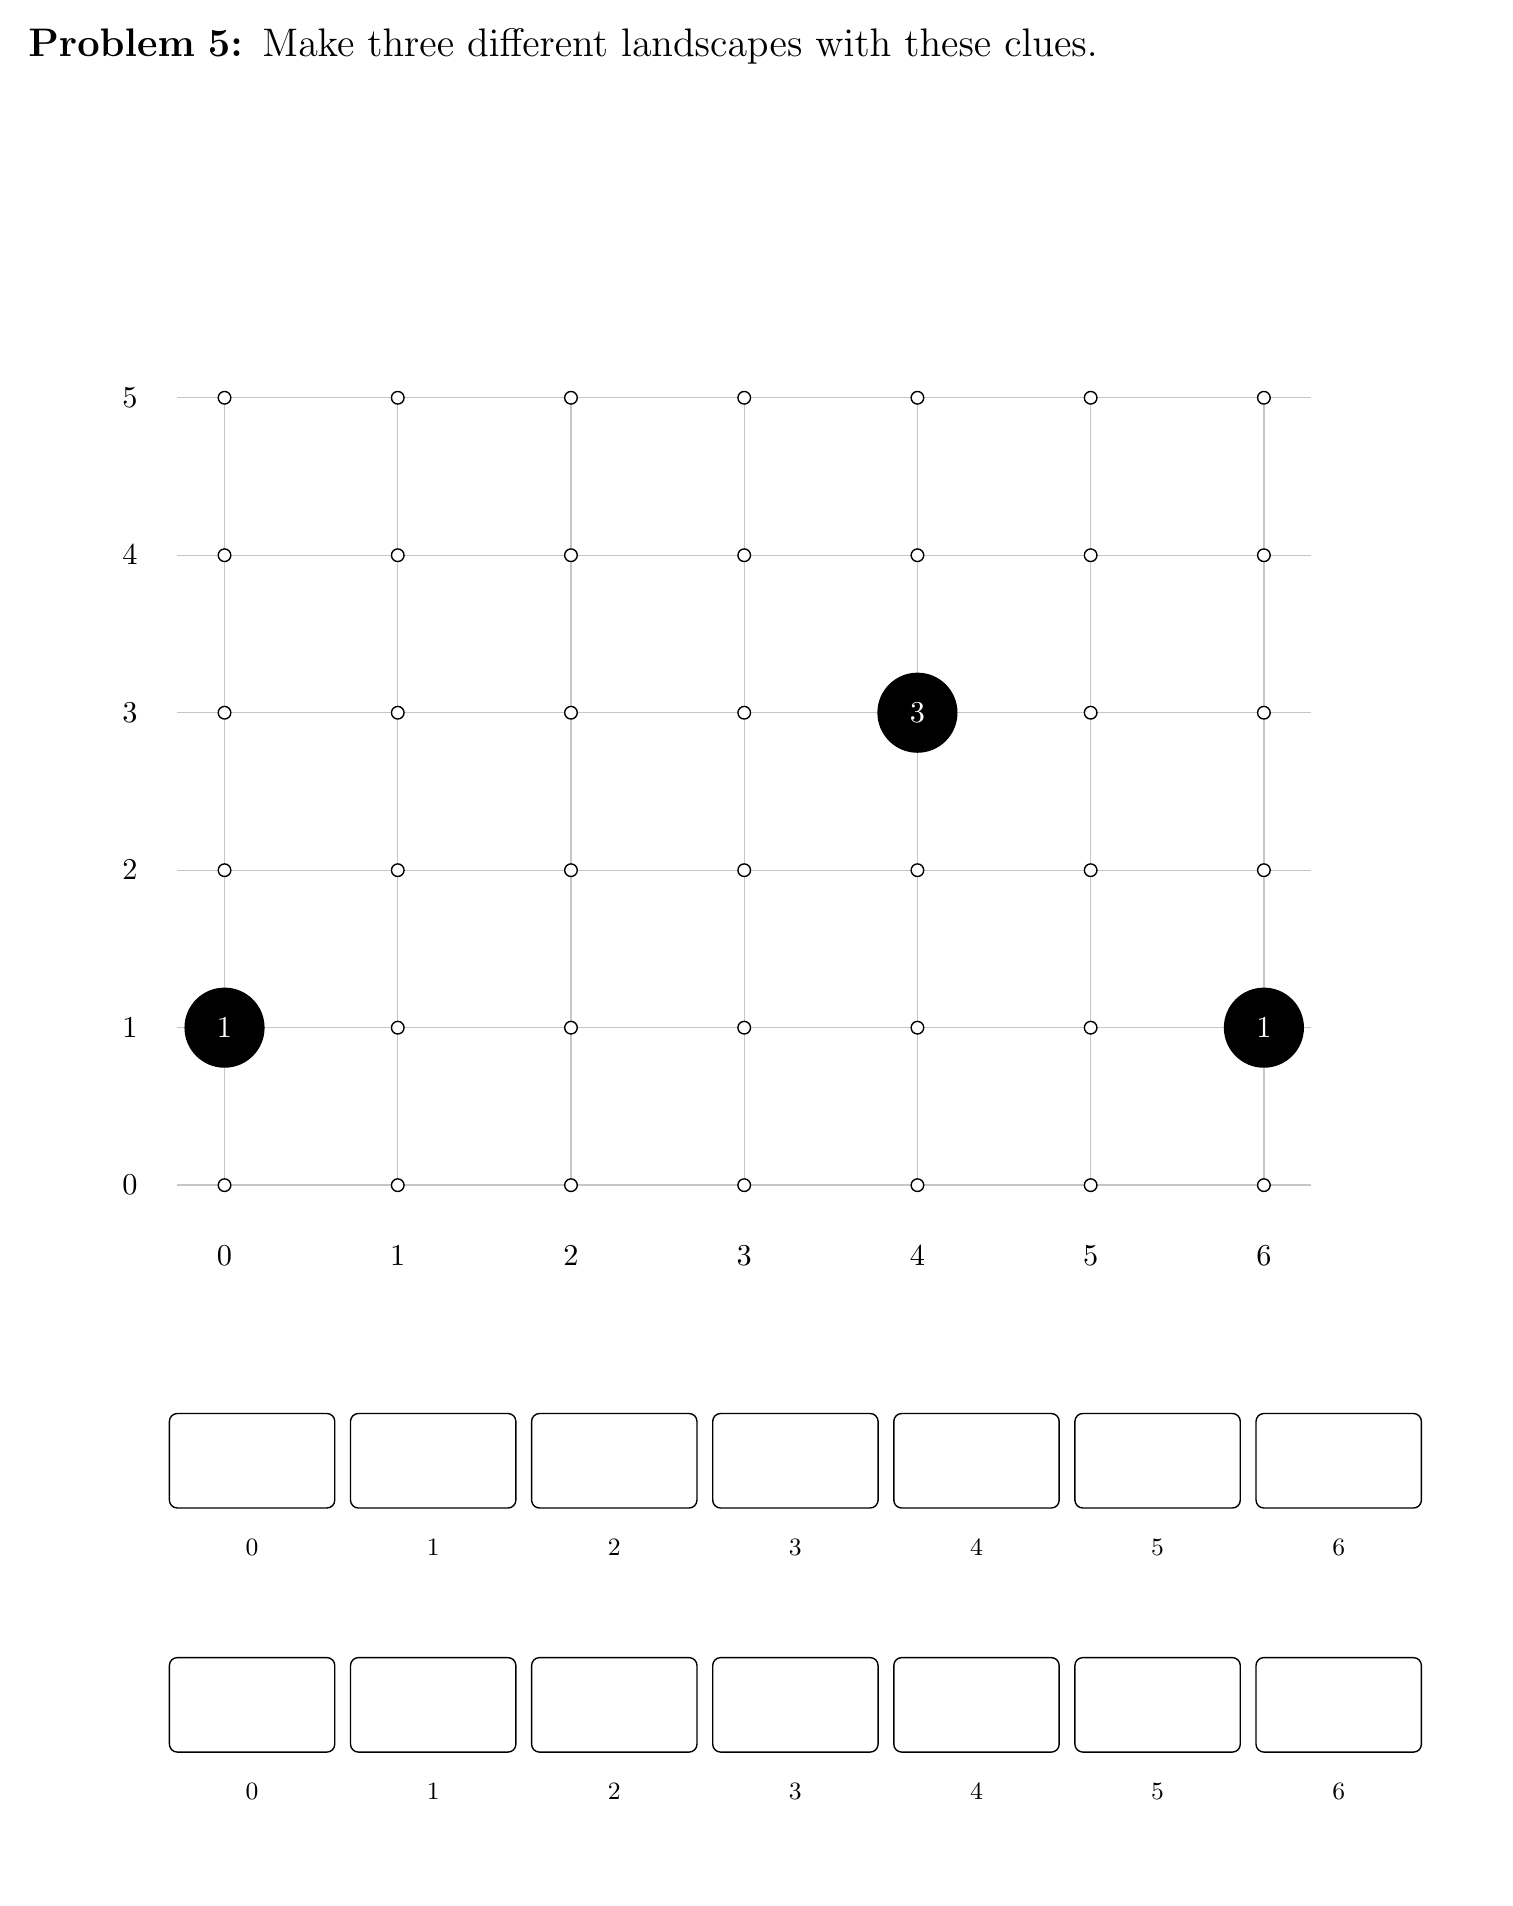
\begin{tikzpicture}[x=1mm,y=-1mm,line width=.5pt]
\path[use as bounding box] (0,0) rectangle (185,235);
\node[anchor=north west,inner sep=0pt,text width=180mm,font=\fontsize{14}{17}\selectfont] at (0,0) {\textbf{Problem 5:} Make three different landscapes with these clues.};
\draw[gray!45] (19,147) -- (163,147);
\node[anchor=center,inner sep=1pt,font=\fontsize{11}{13}\selectfont] at (13,147) {0};
\draw[gray!45] (19,127) -- (163,127);
\node[anchor=center,inner sep=1pt,font=\fontsize{11}{13}\selectfont] at (13,127) {1};
\draw[gray!45] (19,107) -- (163,107);
\node[anchor=center,inner sep=1pt,font=\fontsize{11}{13}\selectfont] at (13,107) {2};
\draw[gray!45] (19,87) -- (163,87);
\node[anchor=center,inner sep=1pt,font=\fontsize{11}{13}\selectfont] at (13,87) {3};
\draw[gray!45] (19,67) -- (163,67);
\node[anchor=center,inner sep=1pt,font=\fontsize{11}{13}\selectfont] at (13,67) {4};
\draw[gray!45] (19,47) -- (163,47);
\node[anchor=center,inner sep=1pt,font=\fontsize{11}{13}\selectfont] at (13,47) {5};
\draw[gray!45] (25,47) -- (25,147);
\draw[fill=white] (25,147) circle (0.8);
\draw[fill=white] (25,127) circle (0.8);
\draw[fill=white] (25,107) circle (0.8);
\draw[fill=white] (25,87) circle (0.8);
\draw[fill=white] (25,67) circle (0.8);
\draw[fill=white] (25,47) circle (0.8);
\node[anchor=center,inner sep=1pt,font=\fontsize{11}{13}\selectfont] at (25,156) {0};
\draw[fill=black] (25,127) circle (5);
\node[anchor=center,inner sep=1pt,font=\fontsize{11}{13}\selectfont] at (25,127) {\color{white}1};
\draw[gray!45] (47,47) -- (47,147);
\draw[fill=white] (47,147) circle (0.8);
\draw[fill=white] (47,127) circle (0.8);
\draw[fill=white] (47,107) circle (0.8);
\draw[fill=white] (47,87) circle (0.8);
\draw[fill=white] (47,67) circle (0.8);
\draw[fill=white] (47,47) circle (0.8);
\node[anchor=center,inner sep=1pt,font=\fontsize{11}{13}\selectfont] at (47,156) {1};
\draw[gray!45] (69,47) -- (69,147);
\draw[fill=white] (69,147) circle (0.8);
\draw[fill=white] (69,127) circle (0.8);
\draw[fill=white] (69,107) circle (0.8);
\draw[fill=white] (69,87) circle (0.8);
\draw[fill=white] (69,67) circle (0.8);
\draw[fill=white] (69,47) circle (0.8);
\node[anchor=center,inner sep=1pt,font=\fontsize{11}{13}\selectfont] at (69,156) {2};
\draw[gray!45] (91,47) -- (91,147);
\draw[fill=white] (91,147) circle (0.8);
\draw[fill=white] (91,127) circle (0.8);
\draw[fill=white] (91,107) circle (0.8);
\draw[fill=white] (91,87) circle (0.8);
\draw[fill=white] (91,67) circle (0.8);
\draw[fill=white] (91,47) circle (0.8);
\node[anchor=center,inner sep=1pt,font=\fontsize{11}{13}\selectfont] at (91,156) {3};
\draw[gray!45] (113,47) -- (113,147);
\draw[fill=white] (113,147) circle (0.8);
\draw[fill=white] (113,127) circle (0.8);
\draw[fill=white] (113,107) circle (0.8);
\draw[fill=white] (113,87) circle (0.8);
\draw[fill=white] (113,67) circle (0.8);
\draw[fill=white] (113,47) circle (0.8);
\node[anchor=center,inner sep=1pt,font=\fontsize{11}{13}\selectfont] at (113,156) {4};
\draw[fill=black] (113,87) circle (5);
\node[anchor=center,inner sep=1pt,font=\fontsize{11}{13}\selectfont] at (113,87) {\color{white}3};
\draw[gray!45] (135,47) -- (135,147);
\draw[fill=white] (135,147) circle (0.8);
\draw[fill=white] (135,127) circle (0.8);
\draw[fill=white] (135,107) circle (0.8);
\draw[fill=white] (135,87) circle (0.8);
\draw[fill=white] (135,67) circle (0.8);
\draw[fill=white] (135,47) circle (0.8);
\node[anchor=center,inner sep=1pt,font=\fontsize{11}{13}\selectfont] at (135,156) {5};
\draw[gray!45] (157,47) -- (157,147);
\draw[fill=white] (157,147) circle (0.8);
\draw[fill=white] (157,127) circle (0.8);
\draw[fill=white] (157,107) circle (0.8);
\draw[fill=white] (157,87) circle (0.8);
\draw[fill=white] (157,67) circle (0.8);
\draw[fill=white] (157,47) circle (0.8);
\node[anchor=center,inner sep=1pt,font=\fontsize{11}{13}\selectfont] at (157,156) {6};
\draw[fill=black] (157,127) circle (5);
\node[anchor=center,inner sep=1pt,font=\fontsize{11}{13}\selectfont] at (157,127) {\color{white}1};
\draw[rounded corners=1mm] (18,176) rectangle ++(21,12);
\node[anchor=center,inner sep=1pt,font=\fontsize{13}{15}\selectfont] at (28.5,182) {};
\node[anchor=center,inner sep=1pt,font=\fontsize{9}{11}\selectfont] at (28.5,193) {0};
\draw[rounded corners=1mm] (41,176) rectangle ++(21,12);
\node[anchor=center,inner sep=1pt,font=\fontsize{13}{15}\selectfont] at (51.5,182) {};
\node[anchor=center,inner sep=1pt,font=\fontsize{9}{11}\selectfont] at (51.5,193) {1};
\draw[rounded corners=1mm] (64,176) rectangle ++(21,12);
\node[anchor=center,inner sep=1pt,font=\fontsize{13}{15}\selectfont] at (74.5,182) {};
\node[anchor=center,inner sep=1pt,font=\fontsize{9}{11}\selectfont] at (74.5,193) {2};
\draw[rounded corners=1mm] (87,176) rectangle ++(21,12);
\node[anchor=center,inner sep=1pt,font=\fontsize{13}{15}\selectfont] at (97.5,182) {};
\node[anchor=center,inner sep=1pt,font=\fontsize{9}{11}\selectfont] at (97.5,193) {3};
\draw[rounded corners=1mm] (110,176) rectangle ++(21,12);
\node[anchor=center,inner sep=1pt,font=\fontsize{13}{15}\selectfont] at (120.5,182) {};
\node[anchor=center,inner sep=1pt,font=\fontsize{9}{11}\selectfont] at (120.5,193) {4};
\draw[rounded corners=1mm] (133,176) rectangle ++(21,12);
\node[anchor=center,inner sep=1pt,font=\fontsize{13}{15}\selectfont] at (143.5,182) {};
\node[anchor=center,inner sep=1pt,font=\fontsize{9}{11}\selectfont] at (143.5,193) {5};
\draw[rounded corners=1mm] (156,176) rectangle ++(21,12);
\node[anchor=center,inner sep=1pt,font=\fontsize{13}{15}\selectfont] at (166.5,182) {};
\node[anchor=center,inner sep=1pt,font=\fontsize{9}{11}\selectfont] at (166.5,193) {6};
\draw[rounded corners=1mm] (18,207) rectangle ++(21,12);
\node[anchor=center,inner sep=1pt,font=\fontsize{13}{15}\selectfont] at (28.5,213) {};
\node[anchor=center,inner sep=1pt,font=\fontsize{9}{11}\selectfont] at (28.5,224) {0};
\draw[rounded corners=1mm] (41,207) rectangle ++(21,12);
\node[anchor=center,inner sep=1pt,font=\fontsize{13}{15}\selectfont] at (51.5,213) {};
\node[anchor=center,inner sep=1pt,font=\fontsize{9}{11}\selectfont] at (51.5,224) {1};
\draw[rounded corners=1mm] (64,207) rectangle ++(21,12);
\node[anchor=center,inner sep=1pt,font=\fontsize{13}{15}\selectfont] at (74.5,213) {};
\node[anchor=center,inner sep=1pt,font=\fontsize{9}{11}\selectfont] at (74.5,224) {2};
\draw[rounded corners=1mm] (87,207) rectangle ++(21,12);
\node[anchor=center,inner sep=1pt,font=\fontsize{13}{15}\selectfont] at (97.5,213) {};
\node[anchor=center,inner sep=1pt,font=\fontsize{9}{11}\selectfont] at (97.5,224) {3};
\draw[rounded corners=1mm] (110,207) rectangle ++(21,12);
\node[anchor=center,inner sep=1pt,font=\fontsize{13}{15}\selectfont] at (120.5,213) {};
\node[anchor=center,inner sep=1pt,font=\fontsize{9}{11}\selectfont] at (120.5,224) {4};
\draw[rounded corners=1mm] (133,207) rectangle ++(21,12);
\node[anchor=center,inner sep=1pt,font=\fontsize{13}{15}\selectfont] at (143.5,213) {};
\node[anchor=center,inner sep=1pt,font=\fontsize{9}{11}\selectfont] at (143.5,224) {5};
\draw[rounded corners=1mm] (156,207) rectangle ++(21,12);
\node[anchor=center,inner sep=1pt,font=\fontsize{13}{15}\selectfont] at (166.5,213) {};
\node[anchor=center,inner sep=1pt,font=\fontsize{9}{11}\selectfont] at (166.5,224) {6};
\end{tikzpicture}
\newpage
\noindent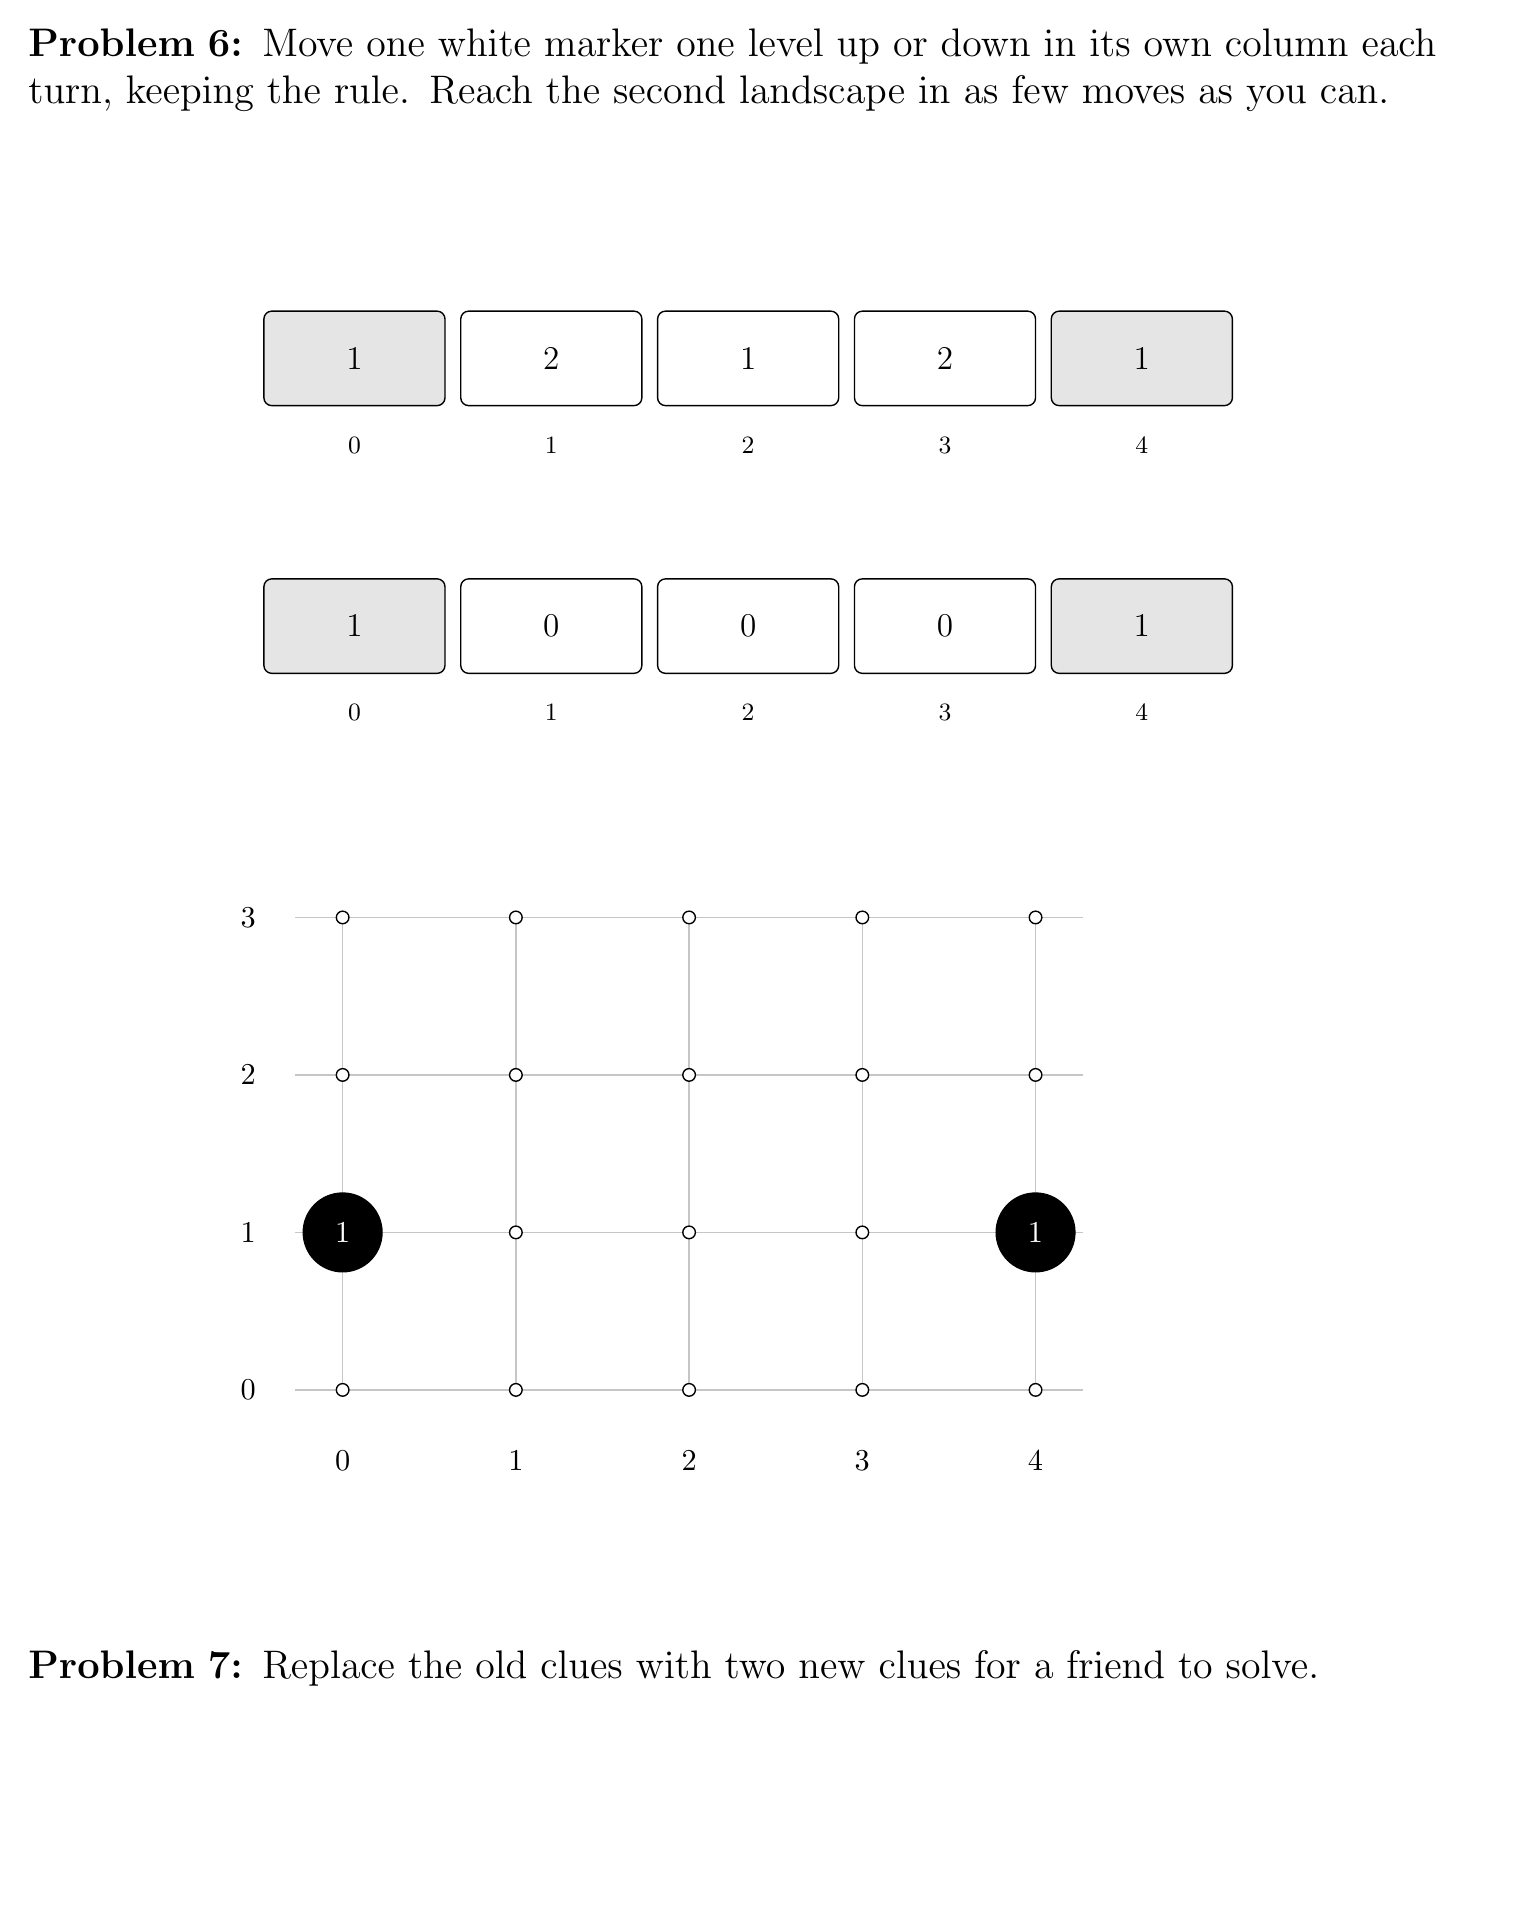
\begin{tikzpicture}[x=1mm,y=-1mm,line width=.5pt]
\path[use as bounding box] (0,0) rectangle (185,235);
\node[anchor=north west,inner sep=0pt,text width=180mm,font=\fontsize{14}{17}\selectfont] at (0,0) {\textbf{Problem 6:} Move one white marker one level up or down in its own column each turn, keeping the rule. Reach the second landscape in as few moves as you can.};
\draw[rounded corners=1mm,fill=gray!20] (30,36) rectangle ++(23,12);
\node[anchor=center,inner sep=1pt,font=\fontsize{13}{15}\selectfont] at (41.5,42) {1};
\node[anchor=center,inner sep=1pt,font=\fontsize{9}{11}\selectfont] at (41.5,53) {0};
\draw[rounded corners=1mm] (55,36) rectangle ++(23,12);
\node[anchor=center,inner sep=1pt,font=\fontsize{13}{15}\selectfont] at (66.5,42) {2};
\node[anchor=center,inner sep=1pt,font=\fontsize{9}{11}\selectfont] at (66.5,53) {1};
\draw[rounded corners=1mm] (80,36) rectangle ++(23,12);
\node[anchor=center,inner sep=1pt,font=\fontsize{13}{15}\selectfont] at (91.5,42) {1};
\node[anchor=center,inner sep=1pt,font=\fontsize{9}{11}\selectfont] at (91.5,53) {2};
\draw[rounded corners=1mm] (105,36) rectangle ++(23,12);
\node[anchor=center,inner sep=1pt,font=\fontsize{13}{15}\selectfont] at (116.5,42) {2};
\node[anchor=center,inner sep=1pt,font=\fontsize{9}{11}\selectfont] at (116.5,53) {3};
\draw[rounded corners=1mm,fill=gray!20] (130,36) rectangle ++(23,12);
\node[anchor=center,inner sep=1pt,font=\fontsize{13}{15}\selectfont] at (141.5,42) {1};
\node[anchor=center,inner sep=1pt,font=\fontsize{9}{11}\selectfont] at (141.5,53) {4};
\draw[rounded corners=1mm,fill=gray!20] (30,70) rectangle ++(23,12);
\node[anchor=center,inner sep=1pt,font=\fontsize{13}{15}\selectfont] at (41.5,76) {1};
\node[anchor=center,inner sep=1pt,font=\fontsize{9}{11}\selectfont] at (41.5,87) {0};
\draw[rounded corners=1mm] (55,70) rectangle ++(23,12);
\node[anchor=center,inner sep=1pt,font=\fontsize{13}{15}\selectfont] at (66.5,76) {0};
\node[anchor=center,inner sep=1pt,font=\fontsize{9}{11}\selectfont] at (66.5,87) {1};
\draw[rounded corners=1mm] (80,70) rectangle ++(23,12);
\node[anchor=center,inner sep=1pt,font=\fontsize{13}{15}\selectfont] at (91.5,76) {0};
\node[anchor=center,inner sep=1pt,font=\fontsize{9}{11}\selectfont] at (91.5,87) {2};
\draw[rounded corners=1mm] (105,70) rectangle ++(23,12);
\node[anchor=center,inner sep=1pt,font=\fontsize{13}{15}\selectfont] at (116.5,76) {0};
\node[anchor=center,inner sep=1pt,font=\fontsize{9}{11}\selectfont] at (116.5,87) {3};
\draw[rounded corners=1mm,fill=gray!20] (130,70) rectangle ++(23,12);
\node[anchor=center,inner sep=1pt,font=\fontsize{13}{15}\selectfont] at (141.5,76) {1};
\node[anchor=center,inner sep=1pt,font=\fontsize{9}{11}\selectfont] at (141.5,87) {4};
\draw[gray!45] (34,173) -- (134,173);
\node[anchor=center,inner sep=1pt,font=\fontsize{11}{13}\selectfont] at (28,173) {0};
\draw[gray!45] (34,153) -- (134,153);
\node[anchor=center,inner sep=1pt,font=\fontsize{11}{13}\selectfont] at (28,153) {1};
\draw[gray!45] (34,133) -- (134,133);
\node[anchor=center,inner sep=1pt,font=\fontsize{11}{13}\selectfont] at (28,133) {2};
\draw[gray!45] (34,113) -- (134,113);
\node[anchor=center,inner sep=1pt,font=\fontsize{11}{13}\selectfont] at (28,113) {3};
\draw[gray!45] (40,113) -- (40,173);
\draw[fill=white] (40,173) circle (0.8);
\draw[fill=white] (40,153) circle (0.8);
\draw[fill=white] (40,133) circle (0.8);
\draw[fill=white] (40,113) circle (0.8);
\node[anchor=center,inner sep=1pt,font=\fontsize{11}{13}\selectfont] at (40,182) {0};
\draw[fill=black] (40,153) circle (5);
\node[anchor=center,inner sep=1pt,font=\fontsize{11}{13}\selectfont] at (40,153) {\color{white}1};
\draw[gray!45] (62,113) -- (62,173);
\draw[fill=white] (62,173) circle (0.8);
\draw[fill=white] (62,153) circle (0.8);
\draw[fill=white] (62,133) circle (0.8);
\draw[fill=white] (62,113) circle (0.8);
\node[anchor=center,inner sep=1pt,font=\fontsize{11}{13}\selectfont] at (62,182) {1};
\draw[gray!45] (84,113) -- (84,173);
\draw[fill=white] (84,173) circle (0.8);
\draw[fill=white] (84,153) circle (0.8);
\draw[fill=white] (84,133) circle (0.8);
\draw[fill=white] (84,113) circle (0.8);
\node[anchor=center,inner sep=1pt,font=\fontsize{11}{13}\selectfont] at (84,182) {2};
\draw[gray!45] (106,113) -- (106,173);
\draw[fill=white] (106,173) circle (0.8);
\draw[fill=white] (106,153) circle (0.8);
\draw[fill=white] (106,133) circle (0.8);
\draw[fill=white] (106,113) circle (0.8);
\node[anchor=center,inner sep=1pt,font=\fontsize{11}{13}\selectfont] at (106,182) {3};
\draw[gray!45] (128,113) -- (128,173);
\draw[fill=white] (128,173) circle (0.8);
\draw[fill=white] (128,153) circle (0.8);
\draw[fill=white] (128,133) circle (0.8);
\draw[fill=white] (128,113) circle (0.8);
\node[anchor=center,inner sep=1pt,font=\fontsize{11}{13}\selectfont] at (128,182) {4};
\draw[fill=black] (128,153) circle (5);
\node[anchor=center,inner sep=1pt,font=\fontsize{11}{13}\selectfont] at (128,153) {\color{white}1};
\node[anchor=north west,inner sep=0pt,text width=180mm,font=\fontsize{14}{17}\selectfont] at (0,206) {\textbf{Problem 7:} Replace the old clues with two new clues for a friend to solve.};
\end{tikzpicture}
\end{document}
